\chapter{Exponentials and Logarithms}
\section{Exponentials}
 An exponential function is a function of the form
 \[f(x)=a^{x},\]
 where $a$ is a positive constant.
 
\begin{example}
\begin{figure}[H]
    \hspace{0.2cm}
    \subfigure[$y=2^x$]{\label{fig:eponential-2-power-x}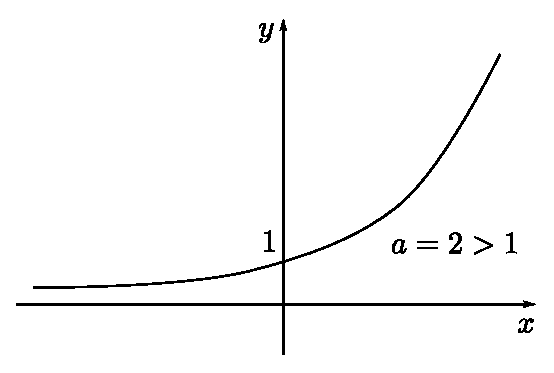
\includegraphics[scale=0.6]{img/eponential-2-power-x}}
    \hspace{2.0cm}
    \subfigure[$y=\left(\frac{1}{2}\right)^x$]{\label{fig:eponential-half-power-x}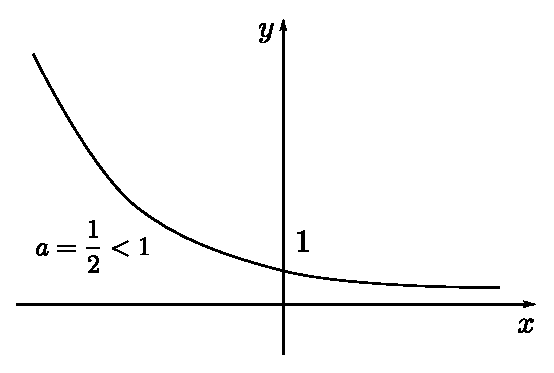
\includegraphics[scale=0.6]{img/eponential-half-power-x}} \\
    \centering
  \caption{Two exponential functions}
  \label{fig:eponential-examples}
\end{figure}
\end{example}

\begin{thing}{Properties}
\begin{enumerate}
 \item[ ] If $a>1$, $f(x)$ increases as $x$ increases.
 \item[ ] If $a<1$, $f(x)$ decreases as $x$ increases.
 \item[ ] If $a=1$, $f(x)=1$.
 \item[ ] $a^0=1$ for each $a$, so the graph always passes through the point $(0,1)$.
\end{enumerate}
\end{thing}
 
\subsection{The gradient of $e^x$}
First let us consider the gradient of $a^x$ at $x=0$. 
\begin{example}
Suppose we have $f(x)=2^x$, then applying the definition of the derivative we have
\[f'(0)=\lim_{h\to0}\frac{f(0+h)-f(0)}{h}=\lim_{h\to0}\frac{2^h-1}{h}.\]
\begin{center}
    \begin{tabular}{ | c | c | }
    \hline
    $h$  & $f'(0)\approx$ \\ \hline
    $0.1$ & $0.7177$ \\ \hline
    $0.01$ & $0.6955$ \\ \hline
    $0.001$ & $0.6933$ \\ \hline
    $0.0001$ & $0.6932$ \\ \hline
    \end{tabular}
\end{center}
%\begin{itemize}
%\item[ ] $h=0.1$ : $f'(0)\approx 0.7177$,
%\item[ ] $h=0.01$ : $f'(0)\approx 0.6955$,
%\item[ ] $h=0.001$ : $f'(0)\approx 0.6933$,
%\item[ ] $h=0.0001$ : $f'(0)\approx 0.6932$.
%\end{itemize}
So for $f(x)=2^x$, ($a=2$), we have slope $\approx0.693$ at $x=0$.
 
Similarly, for $f(x)=3^x$, ($a=3$), we have slope $\approx 1.698$ at $x=0$.
\end{example}

Therefore, we expect that there is a number between 2 and 3 such that the slope at $x=0$ is 1. This number is called $e$, where $e\approx2.718281828459\dots$. The number $e$ is irrational.

\begin{figure}[H]
\centering
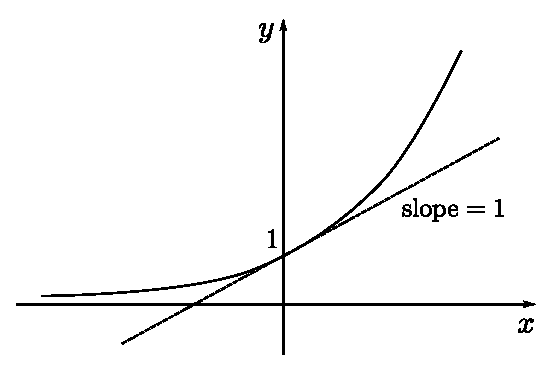
\includegraphics[scale=0.8]{img/graph-exp-x}
\captionstyle{\centering\it}
\caption{Graph of $y=e^x$, which has a gradient of 1 at $x=0$.}
\label{fig:graph-exp-x}
\end{figure}


The fact that the slope is 1 at $x=0$ tells us that
\[\frac{e^h-e^0}{h}=\frac{e^h-1}{h}\to1,\quad \text{as }h\to0.\]

\begin{definition}
We call $f(x)=e^x=\exp(x)$ the \textbf{exponential function}.
\end{definition}

\begin{thing}{Property}
\[\frac{d}{dx}(e^x)=e^x.\]
\begin{proof}
To find the gradient at $x=c$, we need to look at
\begin{align*}
f'(c)&=\lim_{h\to0}\frac{f(c+h)-f(c)}{h}\\
&=\lim_{h\to0}\frac{e^{c+h}-e^c}{h}\\
&=\lim_{h\to0}\frac{e^c(e^h-1)}{h}\\
&=e^c\lim_{h\to0}\frac{e^h-1}{h}\\
&=e^c,\end{align*}
\end{proof}
\end{thing}

\begin{example}
To find $$\frac{d}{dx}\left(e^{\sqrt{1+x}}\right)$$ we must use the chain rule. Choose $g(x)=\sqrt{1+x}$ and $f(u)=e^u$, so we have $g'(x)=\frac{1}{2}(1+x)^{-\frac{1}{2}}$ and $f'(u)=e^u$.
\begin{eqnarray*}
\frac{d}{dx}\left(e^{\sqrt{1+x}}\right) &=& f'(g(x))g'(x) \\
&=& e^{\sqrt{1+x}}\cdot\frac{1}{2}(1+x)^{-\frac{1}{2}} \\
&=& \frac{e^{\sqrt{1+x}}}{2\sqrt{1+x}}.
\end{eqnarray*}
\end{example}

\section{Logarithms}
\begin{definition}
The inverse of an exponenetial function is called a \textbf{logarithm} or \textbf{log}.

The inverse of $a^x$ is written as $\log_a x$ and is defined such that $$a^{\log_a x} = x.$$
\end{definition}
\begin{example}
$\log_{10}(1000)=3$ because $10^3=1000$.

$\log_{2}(16)=4$ because $2^4=16$.

$\log_{10}(2)=0.301...$ because $10^{0.301...}=2$.
\end{example}

\begin{thing}{Laws of Logs}
The following properties hold for logarithms:
\begin{itemize}
\item[1.] $\log_a(MN)=\log_aM + \log_aN$.
\item[2.] $\log_a(M^p)=p\log_aM$.
\end{itemize}
\end{thing}

Logarithms are used among other things to solve exponential equations.

\begin{example}
Find $x$, given $3^x=7$. Taking the logarithm of both sides we have
\[\ln(3^x)=\ln7 \quad \implies \quad x\ln 3=\ln 7.\]
Rearranging we have
\[x=\frac{\ln 3}{\ln 7}\approx\frac{1.95}{1.10}\approx1.77.\]
\end{example}



\subsection{The natural logarithm}
\begin{definition}
The inverse of $f(x)=e^x$ is called the \textbf{natural logarithm} and is written $\ln x$.
\end{definition}

\begin{figure}[H]
    \hspace{0.2cm}
    \subfigure[$y=e^x$.]{\label{fig:exp-x-t-M}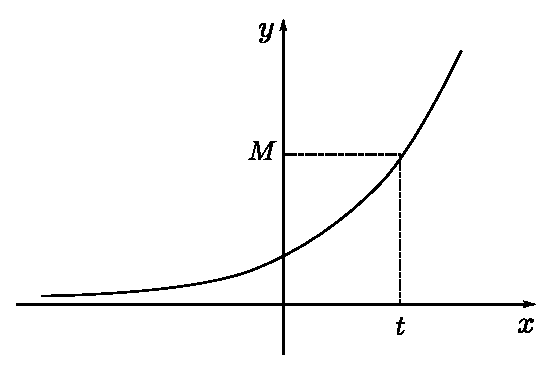
\includegraphics[scale=0.6]{img/exp-x-t-M}}
    \hspace{2.0cm}
    \subfigure[$y=\ln x$.]{\label{fig:log-x-t-M}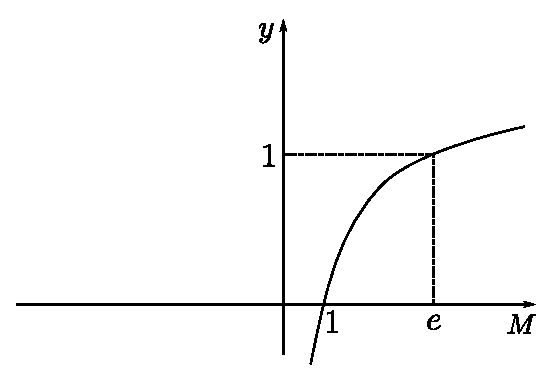
\includegraphics[scale=0.6]{img/log-x-t-M}} \\
    \centering
  \caption{Graphs of the exponential functions and the natural logarithm.}
  \label{fig:exp-log-graphs}
\end{figure}

\begin{thing}{Property}
\[\frac{d}{dx}(\ln x)=\frac{1}{x}.\]
\end{thing}

\begin{example}
To find $$\frac{d}{dx}\left(\ln (\cos x)\right)$$ we must use the chain rule.
Choose $g(x)=\cos x$ and $f(u)=\ln u$, so we have $g'(x)=-\sin x$ and $f'(u)=1/u$. Thus
\begin{eqnarray*}
\frac{d}{dx}(\ln (\cos x)) &=& f'(g(x))g'(x) \\
&=& \frac{1}{\cos x}\cdot (-\sin x) \\
&=& -\tan x.
\end{eqnarray*}
\end{example}
\begin{example}
\begin{eqnarray*}
\frac{d}{dx}(\sin(\ln x)) &=& \cos (\ln x)\cdot\frac{1}{x} \\
&=& \frac{\cos(\ln x)}{x}.
\end{eqnarray*}
\end{example}


\subsection{Differentiation of other logarithms}
\begin{thing}{Property: Change of base}
\[\log_ax=\frac{\log_bx}{\log_ba}\]
In particular, \[\log_ax=\frac{\ln x}{\ln a}.\]
\begin{proof}
Let $$m=\log_ax.$$ This means that $$a^m=x.$$
Applying $\log_b$ to both sides gives:
$$\log_ba^m=\log_bx$$
$$m\log_ba=\log_bx$$
$$m=\frac{\log_bx}{\log_ba}$$

\end{proof}
\end{thing}
\begin{thing}{Property}
\[\frac{d}{dx}\left( \log_ax\right)=\frac{1}{x\ln a}.\]
\begin{proof}
\begin{align*}
\frac{d}{dx}\left(\log_ax\right)
&=\frac{d}{dx}\left(\frac{\ln x}{\ln a}\right)\\
&=\frac{1}{\ln a}\frac{d}{dx}\left(\ln x\right)\\
&=\frac{1}{x\ln a}
\end{align*}

\end{proof}
\end{thing}
%\begin{exer}
%Try to show the above statement is true. Hint: use the chain rule.
%\end{exer}



\section{Differentiation of other exponentials}
\begin{example}
In order to differentiate $3^x$, we must express it in terms of $e^x$:
\[3=e^{\ln 3}\quad \implies\quad 3^x=(e^{\ln 3})^x=e^{x\ln 3}\]
Therefore we calculate the derivative of $3^x$ as follows:
\begin{eqnarray*}
\frac{d}{dx}(3^x) &=& \frac{d}{dx}(e^{x\ln 3}) \\
&=& e^{x\ln 3}\cdot\ln 3 \\
&=& 3^x \cdot \ln 3.
\end{eqnarray*}
\end{example}
\begin{in_a_box}
In general, for any positive constant $a$
\[\frac{d}{dx}(a^x)=a^x\ln a.\]
\end{in_a_box}
